\documentclass[12pt]{article}
\usepackage{amsmath}
\usepackage{amsthm}
\usepackage{amsfonts}
\usepackage{graphicx}
\usepackage{epstopdf}
\usepackage{float}
\usepackage{fancyhdr}
\usepackage{hyperref}
\usepackage{subcaption}
\usepackage{pdfpages}
\usepackage{algpseudocode}
\usepackage{framed}
\usepackage{amssymb}



\makeatletter
\renewcommand\@biblabel[1]{}
\renewenvironment{thebibliography}[1]
     {\section*{\refname}%
      \@mkboth{\MakeUppercase\refname}{\MakeUppercase\refname}%
      \list{}%
           {\leftmargin0pt
            \@openbib@code
            \usecounter{enumiv}}%
      \sloppy
      \clubpenalty4000
      \@clubpenalty \clubpenalty
      \widowpenalty4000%
      \sfcode`\.\@m}
     {\def\@noitemerr
       {\@latex@warning{Empty `thebibliography' environment}}%
      \endlist}
\makeatother

\theoremstyle{definition}
\allowdisplaybreaks
\fancyhf{}


\DeclareMathOperator*{\Max}{Max}
\DeclareMathOperator*{\Min}{Min}
\setlength{\parindent}{0cm}



\begin{document}

\title{Endogenous long-run output impacts of monetary and fiscal policy: a growth theory approach}
\date{}
\author{Daniel H. Stahl}

\maketitle

\newpage
 \begin{abstract}

Traditional economic growth models do not include the impact of government policy on long-run growth.  Conversely, macro-models are often focused on the short-term impacts of government policy in closing an ``output gap'' and don't model the possible long term impacts of government policy on economic output.  In this paper I propose that both monetary and fiscal policy can have long-term impacts on economic growth.  Lower interest rates induce investment in riskier and more entrepeneurial endeavors.  This also causes a shift in labor towards entrepeneural endeavors.  This pool of labor impacts the technological advances which improve the remaining labor's productivity.  Fiscal policy impacts long run growth reducing the economy's effective labor.  This occurs for two reasons: first, the expanded bureaucratic state requires labor to administer.  While this may be a small number relative to the total population, it may have an outsized impact on highly skilled labor.  Second, fiscal policy may dis-incentivize labor participation at the margins, thus reducing output.  I find that, in this model, high rates of interest reduce technological innovation which constrains output per capita to a constant long-run level.  ``Normal'' levels of government spending have mild impacts on output, while high levels may cause output to crash to zero as enough labor is dis-incentived from work.   
\\
\\
Core Results:
\begin{enumerate}
\item Long run growth model incorporates

\end{enumerate}

Keywords: 
\end{abstract}


\newpage
\section{Introduction}

Traditional economic growth models do not include the impact of government policy on long-run growth \cite{solow}. Conversely, macro-models are often focused on the short-term impacts of government policy in closing an ``output gap'' and don't model the possible long term impacts of government policy on economic output \cite{mankiwreis}.  In this paper I propose that both monetary and fiscal policy can have long-term impacts on economic growth.  Lower interest rates induce investment in riskier and more entrepeneurial endeavors.  This also causes a shift in labor towards entrepeneural endeavors.  This pool of labor impacts the technological advances which improve the remaining labor's productivity.  Fiscal policy impacts long run growth reducing the economy's effective labor.  This occurs for two reasons: first, the expanded bureaucratic state requires labor to administer.  While this may be a small number relative to the total population, it may have an outsized impact on highly skilled labor.  Second, fiscal policy may dis-incentivize labor participation at the margins, thus reducing output.  I use an enhanced Solow-style model with a Cobb-Douglas production function which includes monetary and fiscal policy impacts.

\section{Model}

\subsection{Defininitions}
There are three homogenous pools of labor.  \(L_1(t)\) is labor that, combined with capital, produces output.  \(L_2(t)\) is labor that works in research and development.  This labor creates technological efficiencies, \(A(t)\), which enhance the productivity of \(L_1(t)\).  Finally, there is \(L_3(t)\), which is either the ``bureacratic'' labor which maintains the administrative state, or represents capable labor that chooses not to participate in the labor force.  Since \(L_3(t)\) does not impact the output, the model is agnostic to whether labor force participation or bureacratic administration is the primary driver of \(L_3(t)\).  There is capital \(K(t)\).  \(i\) is the interest rate set by the central bank, and \(g\) is the fraction of output that is used for government spending.  It is assumed that this spending is neutral from an output perspective: that is, labor and capital that is employed through fiscal policy has the same output as private sector labor and capital and in the same proportions.
\\
\\
Following Solow \cite{solow}, output \(Y(t)\) takes the following form:

\[Y(t)=K(t)^\alpha (A(t)L_1(t))^{1-\alpha}\]

\subsection{Dynamics}

Total labor \(L(t)=L_1(t)+L_2(t)+L_3(t)\) is constrained by population growth.

\[\frac{dL}{dt}=\eta L(t)\]

\[\frac{dL_3(t)}{dt}=\left(v_0+v_1g\right)L_3(t)\left(1-\frac{L_3(t)}{Y(t)g}\right) \]

Here \(v_0\) is the (presumably small) administrative state in the case of zero government involvement in the economy, and \(v_1\) measures the growth of the administrative state as the government's involvement in the economy grows larger.  This labor is capped by the total government spending in the economy.

\[\frac{dL_2(t)}{dt}=\left(\gamma_0+\gamma_1 (i^*-i) +\gamma_2 g\right) L_2(t) \]

Here \(\gamma_0\) is the non-intervention (baseline) rate of growth in research labor, \(\gamma_1\) is the sensitivity of labor to the prevailing interest rate's deviation from the ``natural'' rate \(i^*\), and \(\gamma_2\) is the proportion of government spending that is dedicated to research and development.  For instance, federal grants to universities would be considered spending on basic research.   
\\
\\
\(L_1\) is determined by the above equations:
\[\frac{dL_1(t)}{dt}=\frac{dL}{dt}-\frac{dL_2(t)}{dt}-\frac{dL_3(t)}{dt}\] 
\[=\eta\left(L_1(t)+L_2(t)+L_3(t)\right)-\frac{dL_2(t)}{dt}-\frac{dL_3(t)}{dt}\]
\\
\\
Technology dynamics are directly proportional to the labor dediated to research.  While in reality research requires some level of capital, the assumption simplifies the analysis.  Many kinds of research (for example, mathematics and economics) requires minimal capital investment.  Of course, the physical sciences often require massive capital investments.  This is a shortcoming of the model.  Note that this also deviates from the classic Solow model where technological growth is exogoneous.
\[\frac{dA(t)}{dt}=\beta L_2(t)\]

Finally, capital follows the familiar dynamics from Solow:
\[\frac{dK(t)}{dt}=s Y(t) - \delta K(t)- L_2(t)\]
\(s\) is the saving rate, \(\delta\) is the rate of capital depreciation, and it is assumed that investment in technology (via \(L_2\)) crowds out investment in capital.  

\subsection{Model analysis}

I focus on output per capita, \(\frac{Y(t)}{L(t)}\). There are three possible long-run states to the model.  First is exponential growth.  This occurs if \(A(t)\) is allowed to grow through time while not crowding out growth in \(L_1(t)\).  The second is a steady state.  This occurs if \(L_2(t)\) shrinks to zero, causing \(A(t)\) to converge to a constant.  The third is economic collapse.  This occurs if \(L_1(t)\) shrinks to zero due to crowding out from \(L_2(t)\) and \(L_3(t)\).  

\subsubsection{Exponential growth}
If \(\eta >\gamma_0+\gamma_1 (i^*-i)+\gamma_2 g > 0\) then \(L_2\) will continue to grow.  This implies that \(A(t)\) will grow without bound, and continued technological growth can continue to provide improved output per capita.  However, this is only the case if both \(L_2(t)\) grows slowly enough to not cause capital to be consumed and \(L_1(t)\) also continues to grow.  

\subsubsection{Steady state}
If \(\gamma_0+\gamma_1 (i^*-i)+\gamma_2 g <0\) then \(L_2(t)\) will shrink to zero and \(A(t)\) will converge to a constant.  If \(L_1(t)\) continues to grow (is not crowded out by \(L_3(t)\)), the economy reaches a long-run steady state in much the same way as the traditional Solow model.

\subsubsection{Economic collapse}
If either \(L_2\) or \(L_3\) grow too large, either \(K\) or \(L_1\) can shrink to zero.  This can occur if interest rates are held too low or \(g\) is too large.  \(L_2\) will grow too quickly if \(\gamma_0+\gamma_1 (i^*-i)+\gamma_2 g > \eta\).  Likewise, \(L_3\) will crowd out \(L_1\) if \(v_0+v_1g > \eta\) and \(g\) IS SOMETHING.

\section{Results}

Since the model is a system of non-linear differential equations, the model must be solved numerically.  I show plots of two economies under different interest rate and fiscal policy regimes.  The full parameters for these two economies:

\begin{center}
\begin{tabular}{ c c c }
      Variable  & Economy 1 Value & Economy 2 Value \\ 
      \(\eta\) & 0.02 & 0.02 \\  
      \(\gamma_0\) & 0.004 & 0.04  \\  
      \(\gamma_1\) & 0.2 & 0.2  \\  
      \(\gamma_2\) & 0.005 & 0.005  \\ 
      \(v_0\) & 0.001 & 0.001  \\  
      \(v_1\) & 0.05 & 0.05  \\  
      \(\beta\) & 0.03 & 0.03  \\  
      \(\alpha\) & 0.4 & 0.4  \\  
      \(\delta\) & 0.1 & 0.1  \\  
      \(s\) & 0.3 & 0.3  \\ 
      \(L_1(0)\) & 3.0 & 3.0  \\ 
      \(L_2(0)\) & 1.0 & 1.0  \\ 
      \(L_3(0)\) & 1.0 & 1.0  \\ 
      \(A(0)\) & 2.0 & 2.0  \\ 
      \(K(0)\) & 10.0 & 10.0  
\end{tabular}
\end{center}

\subsection{Low base growth of research}

In the first economy, the base growth rate of \(L_2\) is low, providing quite a bit of freedom for monetary policy.  

\begin{minipage}[c]{0.8\linewidth}
\begin{framed}
\centering
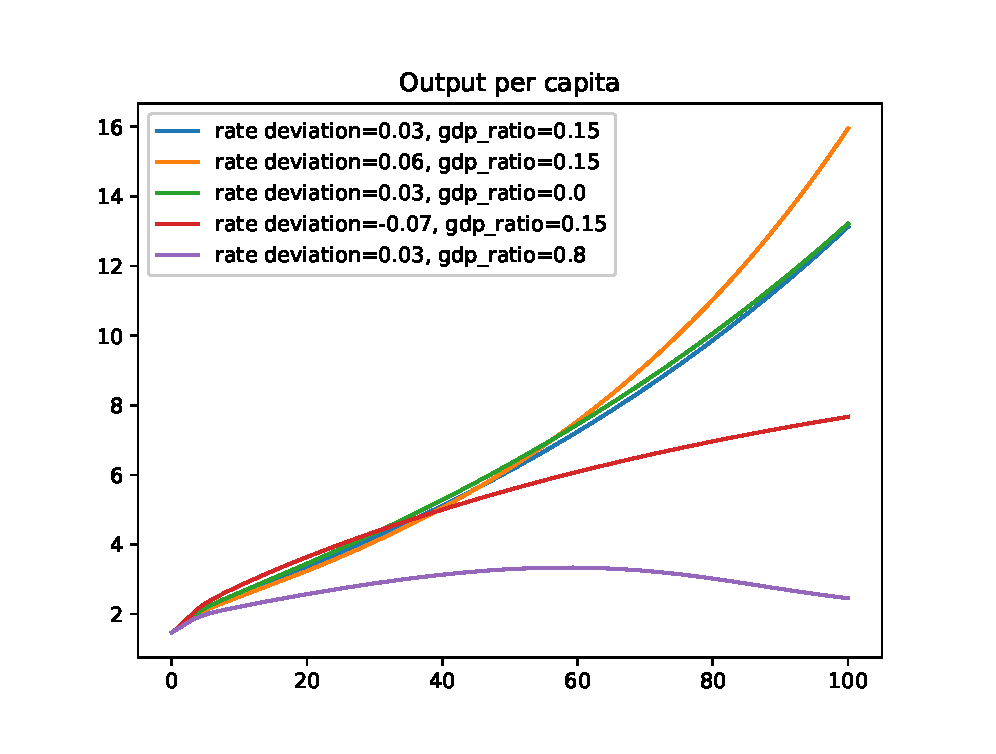
\includegraphics[width=1\textwidth]{images/economy_0}
\end{framed}
\end{minipage}


\begin{minipage}{\linewidth}
\begin{framed}
\begin{minipage}[t]{.48\textwidth}
\centering
\includegraphics[width=1\textwidth]{images/econ_0_run_0_labor}
\end{minipage}\hfill
\begin{minipage}[t]{.48\textwidth}
\centering
\includegraphics[width=1\textwidth]{images/econ_0_run_1_labor}
\end{minipage}\hfill
\begin{minipage}[t]{.48\textwidth}
\centering
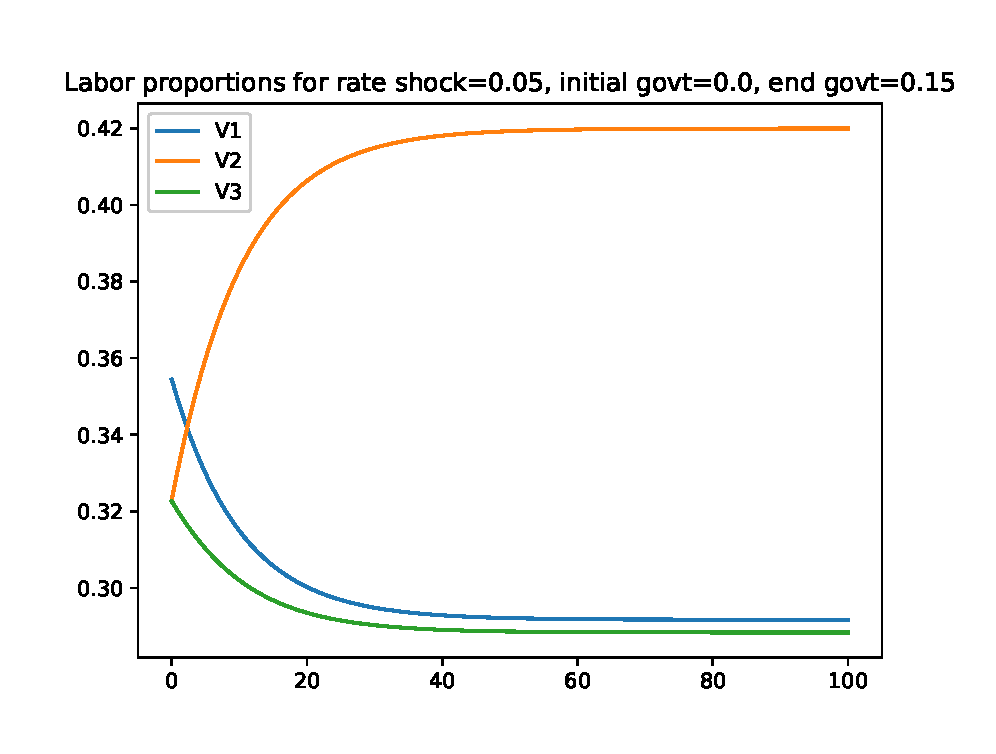
\includegraphics[width=1\textwidth]{images/econ_0_run_2_labor}
\end{minipage}\hfill
\begin{minipage}[t]{.48\textwidth}
\centering
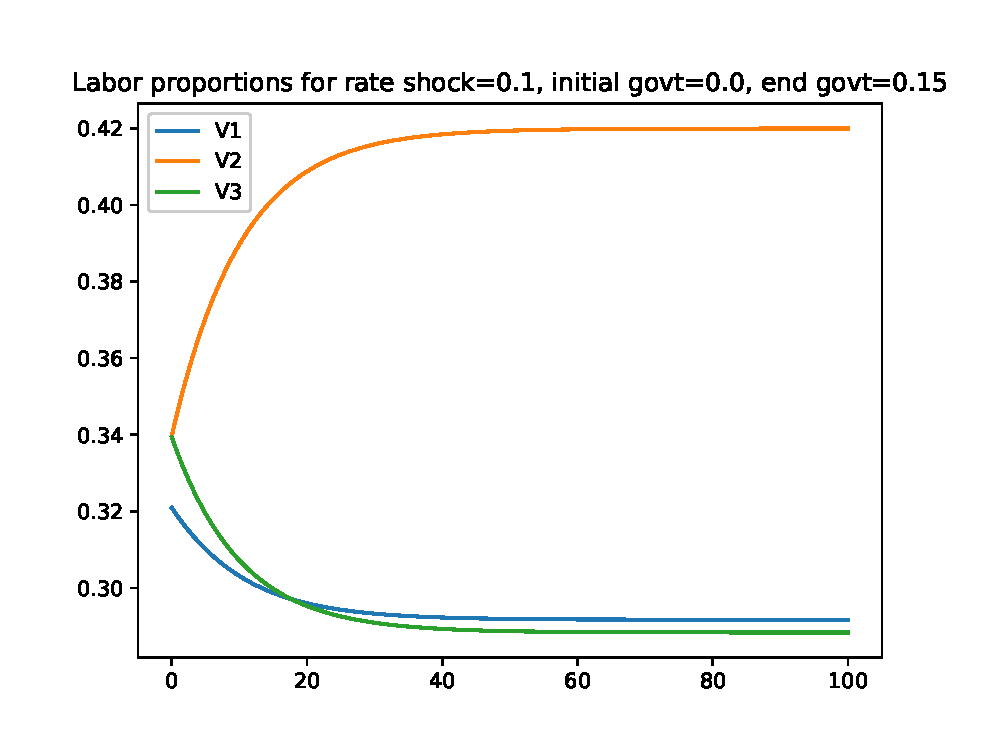
\includegraphics[width=1\textwidth]{images/econ_0_run_3_labor}
\end{minipage} \hfill
\begin{minipage}[t]{.48\textwidth}
\centering
\includegraphics[width=1\textwidth]{images/econ_0_run_4_labor}
\end{minipage}\hfill
\end{framed}
\end{minipage}

The economy becomes stagnant when \(L_2\) goes to zero and collapses when \(L_3\) grows without bound.  For low levels of fiscal involvement there is a tradeoff between the positive impact that fiscal policy has on research and the dicensitives to work and the increased size of the bureaucratic state.  As can be seen with the blue and green lines in the total output chart, the output difference between a 0\% and 15\% fiscal stimulus is very small.  It requires a quite large fiscal ouput (80\% of the economy) to lead to economic collpase.

\subsection{High base growth of research}

In the second economy, the base growth rate of \(L_2\) is high, so that even mild interest rate regimes have deliterious long run impacts.

\begin{minipage}{0.8\linewidth}
\begin{framed}
\centering
\includegraphics[width=1\textwidth]{images/economy_1}
\end{framed}
\end{minipage}


\begin{minipage}{\linewidth}
\begin{framed}
\begin{minipage}[t]{.48\textwidth}
\centering
\includegraphics[width=1\textwidth]{images/econ_1_run_0_labor}
\end{minipage}\hfill
\begin{minipage}[t]{.48\textwidth}
\centering
\includegraphics[width=1\textwidth]{images/econ_1_run_1_labor}
\end{minipage}\hfill
\begin{minipage}[t]{.48\textwidth}
\centering
\includegraphics[width=1\textwidth]{images/econ_1_run_2_labor}
\end{minipage}\hfill
\begin{minipage}[t]{.48\textwidth}
\centering
\includegraphics[width=1\textwidth]{images/econ_1_run_3_labor}
\end{minipage} \hfill
\begin{minipage}[t]{.48\textwidth}
\centering
\includegraphics[width=1\textwidth]{images/econ_1_run_4_labor}
\end{minipage}\hfill
\end{framed}
\end{minipage}

\section{Conclusion}

This model introduced in this paper shows that fiscal and monetary policy can have long run impacts.  

\newpage
\begin{thebibliography}{9}
\bibitem{solow}
R Solow.  A Contribution to the Theory of Economic Growth.  \textit{The Quarterly Journal of Economics}, 70, (1), 1956.
\bibitem{mankiwreis}
N. Gregory Mankiw and Ricardo Reis.  Sticky Information Versus Sticky Prices: A Proposal To Replace The New Keynesian Phillips Curve. \textit{The Quarterly Journal of Economics} 117 (4), 2002.
\end{thebibliography}


\end{document}